\documentclass{article}
\usepackage[utf8]{inputenc}
\usepackage[russian]{babel}
\usepackage[utf8]{inputenc}
\usepackage[T2A]{fontenc}
\usepackage[russian]{babel}
\usepackage{indentfirst}
\usepackage{graphicx}
\usepackage{hyperref}
\usepackage{etoolbox}
\usepackage{float}
\usepackage{wrapfig}
\usepackage{multicol}
\usepackage{multirow,tabularx}
\usepackage{listings}
\usepackage[table,dvipsnames]{xcolor}
\usepackage{soul}
\usepackage{amsmath,amsfonts,amssymb,amsthm}
\usepackage{fp}
\usepackage{array}
\usepackage{adjustbox}
\usepackage{geometry}
\usepackage{amsmath}

\setlength{\parindent}{1.25cm}

\newcommand{\RomanNumeralCaps}[1]
    {\MakeUppercase{\romannumeral #1}}

\begin{document}
\textbf{\S 2. Следящая система с люфтом.} Рассмотрим простейшую
следящую систему с люфтом в контактном устройстве и в зубчатом 
зацеплении, описываемую безразмерным уравнением [152]
\begin{gather}
\ddot{x}+\dot{x}=S(x, \dot{x})
\end{gather}
где $x$ - координата сервомотора и $S(x, \dot{x})$ - кусочно-постоянная
(характеризующая безразмерную э. д. с. и сухое трение в системе). 
Общеизвестным приемом при исследовании точечных преобразований 
является представление и исследование точечного преобразования в 
параметрической форме, где в качестве параметра вводится время пробега 
изображающей точки по траекториям системы между точками сшивания.%abzac

Особенностью рассматриваемой задачи является возможность
другого эффективного параметрического представления точечного
преобразования с введением в качестве параметров некоторых
отрезков в фазовом пространстве. Этот прием имеет значение, вы
ходящее за рамки рассматриваемой задачи.%abzac

Разбиение плоскости $(x, \dot{x})$ на области, где $C(x, \dot{x})$ сохраняет
постоянное значение, производится в зависимости от двух параметров 
$k$ и $z$, характеризующих соответственно люфт в котактном 
устройстве и люфт в зацеплении.%abzac

Запишем уравнение (1) в виде системы
\begin{gather}
\dot{x}=y, \quad \dot{y}=S(x,y)-y
\end{gather} 
и будем рассматривать фазовые траектории на плоскости $(x, y)$.
Разбиение фазовой плоскости на траектории будет симметрично
относительно начала координат, если за начало отсчета 
\begin{wrapfigure}{r}{0.5\textwidth}

\raggedleft

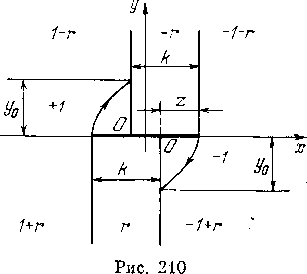
\includegraphics[width=1\linewidth]{../img/img210.png}

%\caption{Рис. 210}

\label{fig:mpr}

\end{wrapfigure}
принять середину максимального интервала 
длиной $z+k$, который сервомотор
 может пройти по инерции. На
рис. 210 изображено разбиение
плоскости $(x, y)$ на десять областей,
где $S(x, y)$ сохраняет
постоянные значения, указанные 
на рисунке. Полосы шириной 
$y0$, примыкающие к оси $x$
сверзу или снизу, соответствуют
выбиранию сервомотором люфта
в зубчатом зацеплении, и для
них соответственно $S(x, y)=1$
или $S(x, y)=-1$ (сухим трением
при свободном движении сервомотора пренебрегаем). Полосе шириной $k$, содержащей внутри ось $y$, соответствует выбирание сервомотором совместно со следящей осью люфта в коптактном
устройстве при движении по инерции. Здесь $S(x, y)=-r$ или
$S(x, y)=r$ характеризует твердое трение в системе. На других
участках фазовой плоскости величина $S(x, y)$ имеет значение
$\pm 1 \pm r$, где знаки выбираются в зависимости от знака скорости
и знака включенной э. д. с. или 0, если люфт в зацеплении про
ходится по инерции. Величина $y_{0}$-максимаьная скорость, до
которой разгоняется сервомотор, выбирая люфт в зацеплении,
есть однозначная функция параметра $z$ и определяется уравнением
\begin{gather}
z+y_{0}+ln(1-y_{0})=0.
\end{gather}
Это уравнение получатется, если в (2) положить $S(x,y)=1$ и
потребовать для решения системы (2) выполнения условий $x=$
$=-x_{0}, y=0; x=-x_{0}+z, y=y_{0}$.%abz

Построим точечное преобразование в себя полупрямой $L:$
$y=0, x\leq\frac{-(z+k)}{2}$, примыкающей слева к отрезку покоя: $y
=0, \frac{-(z+k)}{2}<x<\frac{z+k}{2}$. Так как фазовое пространство
симметрично оносительно начала координат, то задача сводится
к построению точечного отображнеия полупрямой $L$ в симметричную 
полупрямую $L'$, примыкающую к отрезку покоя справа.%абзац

Рассмотрим траекторию в верзней полуплоскости, сшитую из
четырех ксков, начинающуюся в точке $(-u, 0)$ и заканчиваю
щуюся в точке $(v,0)$. \flqq Сшивание \frqq траекторий в точках разрыва 
правых частей системы совершается элементарно, если знак
правой части второго из уравнений (2) не изменяется при переходе 
через линию сшивания. Так будет, если $y_{0}\leq1-r$, т. е. если
$r$ "не слишком велико". Точки пересечения этой траектории с по
лосой ширины $k$ будут $x=\frac{z-k}{2}, y=\eta$ и $x=\frac{z+k}{2}, y=x_{i}$. Как
оказывается, величины $\eta$ и $\xi$ целесообразно рассматривать как
параметры точечного преобразования.%абзац

Из уравнения (2), полагая $S(x, y)=1$ для первого куска
траектории и $S(x, y)=1-r$ для второго и используя условия
для концов кусков траекторий: $x=-u, \, y=0; \, x=-u+z, \, y=y_{0};$
$x=\frac{z-k}{2} \, y=r_{i}$, получим
\begin{gather}
u=\frac{z+k}{2} + (1-r) \, ln\frac{1-r-y_{0}}{1-r-\eta}+y_{0}-\eta, \quad  y_{0}\leq\eta<1-r.
\end{gather}
Полагая далее $S(x,y)=-r$ для третьего куска траектории и
$S(x,y)=-1-r$ для четвертого и используя условия для концов
кусков траекторий
\begin{center}
$x=\frac{z-k}{2}, \quad y=\eta; \quad x=\frac{z+k}{2}, \quad y=\xi; \quad x=v,  \quad y=0,$
\end{center}
получим
\begin{gather}
r ln(\xi + r) - r ln(\xi+r)+\eta-\xi-k=0,
\end{gather}
\begin{gather}
v=\frac{z+k}{2}+\xi+(1+r)ln\frac{1+r}{\xi+1+r}, \quad 0\leq\xi<\infty. 
\end{gather}
Уравнения (4)-(6) определяют требуемое точечное преобразование 
в параметрической форме с двумя параметрами $\eta$ и $\xi$.
Разбиение фазового пространства $(x,y)$ на траектории определяется 
взаиморасположением кривых $u=u(\eta)$ и $v=v(\eta)$ на совмещенных 
плоскостях $(\nu, u)$ и $(\nu, v)$. Исследование взаиморас
положения кривых проводится элементарно при использовании
$\eta$ и $\xi$ как параметров.%абзац

Из (5) и(6) находим
\begin{center}
$\frac{d\eta}{d\xi}=\frac{\xi(\eta+r)}{\eta(\xi+r)}> 0, \quad \frac{dv}{d\xi}=\frac{\xi}{\xi+1+r}>0.$
\end{center}
Откуда
\begin{gather}
\frac{dv}{d\eta}=\frac{\eta}{1+r+\xi} \, \frac{\xi+r}{\eta+r}>0.
\end{gather}
Из (4) имеем\\%абзац
\begin{gather}
\frac{du}{d\eta}=\frac{\eta}{1-r-\epsilon}.
\end{gather}
Сравнивая (7) и (8), непосредственно обнаруживаем, что для
любого $\eta$ будет
\begin{center}
$du/d\eta>dv/d\eta$,
\end{center}
и, следовательно, если существует точка пересечения кривых
$u=u(\eta)$ и $v=v(\eta)$, то она единственная и соответствует устойчивой,
неподвижной точке преобразования.

Граничные значения кривых $u=u(\eta)$ и $v=v(\eta)$ будут
\begin{center}
$u=(z+k)/2, \quad v=(z+k)/2$
\end{center}
соответственно при значениях параметров $\eta=y_{0}$и $\eta=y_{1}$ ($y_{1}$ определяется 
как корень уравнения (5) при $\xi=0$).

Для значений $\eta$, близких к $1-r$ ($ \eta=1-r$ - асимптота для
$u=u(\eta)$), будет $u>v$. Точка пересечения кривых $u=u(\eta)$ и

\begin{wrapfigure}{r}{0.3\textwidth}

\raggedleft

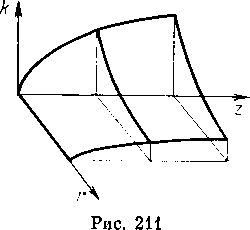
\includegraphics[width=1\linewidth]{../img/img211.png}

%\caption{Рис. 210}

\label{fig:mpr}

\end{wrapfigure}

$v=v(\eta)$, будет поэтому существовать,
если $y_{1}<y_{0}$. Граница области существования
неподвижной точки преобразования
и соответствующего ей устойчивого
предельного цикла определяется
условием $y_{1}=y_{0}$.

Уравнение (3) совместно с уравнением
\begin{gather}
r \, ln \, r - r \, ln(y_{0}+r)+y_{0}-k=0,
\end{gather}
полученным из (5) при $\xi=0$ и $\eta=y_{0}$,
дает в параметрической форме уравнени
поверхности (рис. 211), отделяющей в пространстве параметров
область автоколебаний от области абсолюной устойчивости.
Точкам ниже поверхности соответствует область
автоколебаний. Точкам выше поверхности - устойчивость
в большом (рис. 212, \textit{а}). Точкам по поверхности - 
\begin{figure}[h]

\centering

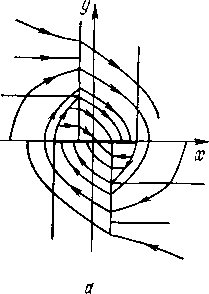
\includegraphics[width=0.3\linewidth]{../img/img212__1.png}
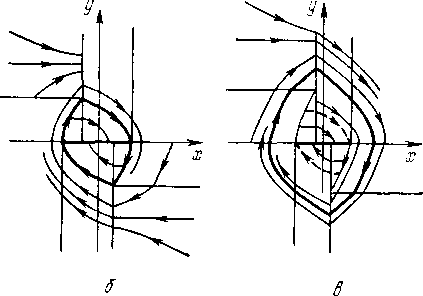
\includegraphics[width=0.6\linewidth]{../img/img212__2.png}

\setcounter{figure}{1}
\renewcommand{\thefigure}{212}

\caption{}

\label{ris:image}



\end{figure}
вырожденный двойной цикл, проходящий через концы отрезка покоя
(рис. 212, \textit{б}). На рис. 212, \textit{в} изображены два склеенных предельных
цикла - устойчивый и неустойчивый (неустойчивый обозначен
штриховой линией).

Если $r$ \flqq велико \frqq ($y_{0}>1-r$), фазовые траектории подходят с 
обеих сторон к линиям сшивания $y=\pm y_{0}$и система (2) должна
быть из физических соображений доопределена условием
\begin{center}
$$
\dot{x}=y, y=
\left\{
    \begin{array}{ll}
        &y_{0}  \mbox{ при } x \leq -(z-k)/2,\\
        -&y_{0}  \mbox{ при } x \geq (z-k)/2,
    \end{array}
\right.
$$
\end{center}
требующим, чтобы движение продолжалось по линии стыков таекторий
(скользящий режим). Уравнение (4) теряет сысл. Любая 
траектория, сшитая из четырех кусков в верхней полуплоскости,
начинающаяся в точке $(-u, 0)$ и заканчивающаяся в точке
$(v, 0)$, содержит кусок прямой $y=y_{0}$, принадлежащий линии
сшивания. В уравнении (5) праметр $\eta$ принимает фиксорованное
значение $y_{0}$. Уравнения (5) и (6) будут в параметрическом
виде (с параметром $\xi$) связывать $v$ и $k$. Уравнение (9) сохраняет
\begin{figure}[h]

\centering

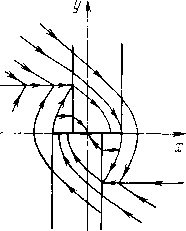
\includegraphics[width=0.3\linewidth]{../img/img213__1.png}
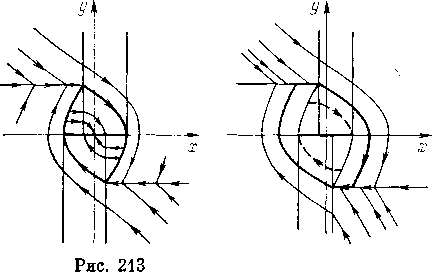
\includegraphics[width=0.6\linewidth]{../img/img213__2.png}

\label{ris:image}

\end{figure}
смысл и для случая сколь угодно больших $r$.

На рис. 213 изображены различные возможные тиы разбиения фазовой плоскости
для этого случая. В отличие от случая \flqq малых $r$ \frqq, здесь устойчивый
предельный цикл будет вырожденным (на него переходят
точки сконтинуума траекторий).

\textbf{\S 3. Электрическая цепь с туннельным диодом.} Рассматривается
 система [28]
\begin{gather}
\dot{x}=y-\phi(x), \quad \dot{y}=\sigma - \lambda x-y, \quad g>0, \quad \lambda>0,
\tag{1}
\end{gather}
где $\phi$ - нелинейная  функция, содержащая \flqq падающий \frqq участок.
Система такого вида встречается при рассмотрениисхем на 
туннельных диодах, а также в ряде других вопросов. Аппроксимируем
$\phi(x)$ кусочно-линейной функцией, состоящей из трех линейных
кусков. наклоны $k$ будем считать: падающего участка
$k=-\alpha_{2}<0$, восходящих $k=\alpha_{1}>0$. Фазовое пространство при
такой аппроксимации разбивается на три части, в каждой из которых
система линейна. В областях \RomanNumeralCaps{1} и \RomanNumeralCaps{3} лежат восходящие
ветви характеристики, в области \RomanNumeralCaps{2} - падающий участок (рис. 214).

\textbf{1. Состояния равновесия. Разбиение пространства параметров
по числу и характеру состояний равновесия.} Возможны одно
или три грубых состояния равновесия. В случае одного состояния
равновесия имеем фокус (узел), всегда устойчивый в областях
\RomanNumeralCaps{1} или \RomanNumeralCaps{3} и неустойчивый в области \RomanNumeralCaps{2}, если $\alpha_{2}>1$. В случае
\begin{wrapfigure}{r}{0.5\textwidth}

\raggedleft

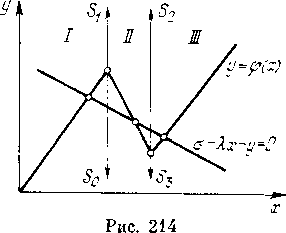
\includegraphics[width=1\linewidth]{../img/img214.png}

%\caption{Рис. 210}

\label{fig:mpr}

\end{wrapfigure}
трех состояний равновесия имеем
всегда устойчивые фокусы (узлы)
в областях \RomanNumeralCaps{1} и \RomanNumeralCaps{3} и седло в области
\RomanNumeralCaps{2}. Куски прямых $\sigma = x_{1} \lambda +y_{1}$
и $\sigma = x_{2} \lambda +y_{2}$ ($x_{1}, y_{1}$ и $x_{2},$
$y_{2}$ - координаты угловых точек
характеристики) при $\lambda \leq \alpha_{2} $ образуют
в плоскости $(\lambda, \sigma)$ дискриминантную 
кривую, отделяющую область
трех состояний равновесия
от области одного состояния равновесия. Точкам дискриминантной
кривой соответствует сшитое состояние
равновесия типа седло-фокуса или седло-узла, и уговой 
точке $(\lambda = \alpha_{2})$ - неустойчивый отрезок покоя, совпадающий с падающим
участком арактеристики.

В случа $\alpha_{2}<1$ невозможны замкнутые траектории и возможными
бифуркациями являются только появлиние и исчезновение
состояний равновесия. Все нижеследующие рассмотрения ведутся
для случая $\alpha_{2}>1$ и $(\alpha - 1)^2<4a_{2}$, допускающего разнообразные
бифуркации.

\textbf{2. Бифуркации состояний равновесия.}

2.1 \textit{Устойчивость состояния равновесия на линии сшивания.}
Пусть прямая $\sigma - \lambda x - y = 0$ проходит через угловую точку
$(x_{1}, y_{1})$ характеристики на границе \RomanNumeralCaps{1} и \RomanNumeralCaps{2} областей и пусть
$\lambda > (\alpha_{2} + 1)^2/4>\alpha_{2}$. Тогда область \RomanNumeralCaps{1} заполнена кусками траекторий 
устойчивого фокуса, а область \RomanNumeralCaps{2} - неустойчивого. Вводим на 
линии сшивания областей \RomanNumeralCaps{1} и \RomanNumeralCaps{2} положительные координаты $S_{0}$ 
и $S_{1}$ (а на линии сшивания областей \RomanNumeralCaps{2} и \RomanNumeralCaps{3} - координаты $S_{2}$ и 
$S_{3}$) (см. рис. 214). Преобразования $S_{0} \rightarrow S_{1}$ по траекториям области
\RomanNumeralCaps{1} и $S_{1} \rightarrow S_{0}$ по траекториям области \RomanNumeralCaps{2} запишутся так:
\begin{gather}
S_{2}=S_{0} \, exp \, \{-h_{1}\pi/ \omega_{1}\}, \overline{S}_{0}=S_{1} \, exp \, \{-h_{2}\pi / \omega_{2}\},
\tag{2}
\end{gather}
где $\omega_{i}, \, -h_{i}  \, (i=1, 2)$ - мнимая и действительная части корней
характеристического уравнения соответственно для областей
\RomanNumeralCaps{1} и \RomanNumeralCaps{2}.

Состоянием равновесия будет сшитый цетр $(\overline{S}_{0}=S_{0})$, если 
$h_{1} \omega_{1}^{-1} + h_{2}^{-1} \omega_{2}^{-1}=0$ или, в раскрытом виде,
\begin{center}
$\lambda=\lambda^+ \equiv (\alpha_{1} \alpha_{2} + 1)(\alpha_{1} - \alpha_{2} + 2)^{-1}$.
\end{center}
Фокус на склейке будет устойчив $(\overline{S}_{0}<S_{0})$ при $\lambda > \lambda^+$ и неустойчив
$(\overline{S}_{0}>S_{0})$ при $\lambda<\lambda^+$.

2.2 \textit{Рождение предельного цикла из состояния равновесия типа
фукос при перемещении состояния равновесия через линию 
сшивания.} Докажем, что в областях \RomanNumeralCaps{1} и \RomanNumeralCaps{2} может существовать не более одного предельного цикла. Рассмотрим преобразование
$S_{0} \rightarrow \overline{S}_{0}$ по траекториям областей \RomanNumeralCaps{1} и \RomanNumeralCaps{2}. Для области \RomanNumeralCaps{1} будет
\begin{center}
$S_{0} = \frac{\delta_{0}}{\sin \omega_{1} \tau_{1}} [ \omega_{1} \cos \omega_{1} \tau_{1} + h_{1} \sin \omega_{1} \tau_{1} - \omega_{1} $
$e^{h_{1} \tau_{1}} ] = \delta_{0} \xi (\tau_{1}), $
\end{center}
\begin{gather}
S_{1} = \frac{\delta_{0}}{\sin \omega_{1} \tau_{1}} [ \omega_{1} \cos \omega_{1} \tau_{1} - h_{1} \sin \omega_{1} \tau_{1} - \omega_{1}e^{-h_{1} \tau_{1}} ] = \delta_{0} \chi (\tau_{1}),
\tag{3}
\end{gather}
где $\delta_{0}$ - расстояние от границы раздела областей \RomanNumeralCaps{1} и \RomanNumeralCaps{2} до состояния
равновесия; $\chi$ и $\xi$ - монотонные функции (возрастающие
или убывающие в зависимости от знака $\delta_{0}$). Преобразование 
по траекториям области \RomanNumeralCaps{2} записывается аналогично.

Вычисление производной функции последования дает
\begin{gather}
d\overline{S}_{0}/dS_{0} = S_{0}\overline{S}_{0}^{-1} exp\{-2(h_{1} \tau_{1} + h_{2} \theta)\}.
\tag{4}
\end{gather}
Здесь $\tau$ и $\theta$ - время движения соответственно по траекториям
областей \RomanNumeralCaps{1} и \RomanNumeralCaps{2}, $h_{1}=(1 + \alpha_{1})/2 > 0, h_{2}=(1 - \alpha_{2})/2 < 0$.

Пусть состояние равновесия лежит в области \RomanNumeralCaps{1}. Тогда для переодического 
решения $(\overline{S}=S_{0})$ с увеличением $S_{0}$ время $\tau_{1}$ убывает
(до значения $\pi / \omega_{1}$), время $\theta$ возрастает (до значения $\pi / \omega_{2}$)
и производная (4) растет. Поэтому может существовать не более 
двух точек пересечения функции последования с биссектрисой,
причем неподвижная точка с меньшей координатой должна быть
устойчива, а с большей - неустойчива. Так как, по предположению,
состояние равновесия лежит в области \RomanNumeralCaps{1} и является устойчивым фокусом, который не может охватываться усттойчивым же
циклом, то в областях \RomanNumeralCaps{1} и \RomanNumeralCaps{2} может существовать не более одного,
причем неустойчивого цикла.

Пусть состояние равновесия лежит в области \RomanNumeralCaps{2}. Тогда с ростом
$S_{0}$ время $\tau_{1}$ растет, а $\theta$ убывает. Аналогично находим, что
в этом случае может существовать не более одного устойчивого 
предельного цикла.

Пусть $\sigma - \lambda x - y = 0$ проходит через верхнюю угловую точку
характеристики. Рассмотрим два случая.

1. $\lambda > \lambda^+$. Сшитый фокус устойчив. траектория, проходящая 
через нижнюю угловую точку, в силу (2) при $t \rightarrow \infty$ накручивается
к состоянию равновесия. Эта траектория остается спиралью
и при малых смещениях прямой $\sigma - \lambda x - y = 0$. Если при
малом смещении состояние равновесия попадает в область \RomanNumeralCaps{2}, то
оно становится неустойчивым и, следовательно, появляется хотя
бы один устойчивый предельный цикл. По сказанному выше этот
цикл единственный. Пусть после смещения состояние равновесия
попадает в область \RomanNumeralCaps{1}. так как в объединении областей \RomanNumeralCaps{1} и \RomanNumeralCaps{2} возможно
существование не более одного цикла и фокус сохраняет
устойчивость, то, следовательно, циклы не возникают.

2. $\lambda < \lambda^+$. Аналогично находим, что если при малом смещении
состояние равновесия попадает в область \RomanNumeralCaps{2}, то циклы не возникают, 
а если в область \RomanNumeralCaps{1}, то появляется неустойчивый цикл.

2.3 \textit{Рождение предельных циклов (простого или двойного) из
границы области, заполненной замкнутыми траекториями.} Рассмотрим
преобразования $\overline{S}_{0}=f(S_{0})$, склеенные из двух кусков:
$\overline{S}_{0}= \phi(S_{0})$ - по траекториям областей \RomanNumeralCaps{1} и \RomanNumeralCaps{2} и $\overline{S_{0}}=\psi(S_{0})$ - по всем
областям. Покажем, что $f(S_{0})$, дифференцируема в точке склейки.
Преобразование $S_{0} \rightarrow S_{1}$, по траекториям области \RomanNumeralCaps{1} дано в (3).
Преобразования $S_{1} \rightarrow S_{2}, S_{2} \rightarrow S_{3}$ и$ S_{3} \rightarrow S_{0}$ записываются аналогично.
Значение $d\overline{S}_{0}/dS_{0}$ для функции $\psi(S_{0})$ дано в (4), а для 
функции $\psi(S_{0})$ будет
\begin{gather}
d\overline{S}_{0}/dS_{0} = S_{0}\overline{S}_{0}^{-1} \, exp \{-2h_{1}(\tau_{1} + \tau_{3}) - 2h_{2}(\tau_{2} + \tau_{4})\}.
\tag{5}
\end{gather}
Здесь $\tau_{1}$ и $\tau_{3}$ - время движения по областям \RomanNumeralCaps{1} и \RomanNumeralCaps{3}, $\tau_{2}$ и $\tau_{4}$ - время движения по верзу и низу области \RomanNumeralCaps{2}.

Пусть $S_{0}=S_{0}^*$ - граничное значение, разделяющее интервалы
определения преобразований $\phi(S_{0})$ и $\psi(S_{0})$. Производные для 
$\phi$ и $\psi$ в точке склейки совпадают: при $S = S_{0}^*$ будет $\tau_{3} = 0, \theta = \theta^*$,
$\tau_{2} + \tau_{4} = \theta^*$.

Пусть теперь прямая $\sigma - \lambda x - y = 0$ проходит через угловую точку характеристики $x_{1}, y_{1}$ и $\lambda = \lambda^+$. Покажем, что предельных
циклов нет.

Функция последования на плоскости $(S_{0}, \overline{S}_{0})$ склеена из отрезка
биссектрисы $\overline{S}_{0} = S_{0} < S_{0}^*$ и кривой $\overline{S}_{0} = \psi(S_{0})$. Функция
$\overline{S}_{0} = f(S_{0})$ дифференцирума в точке склейки и, следовательно,
при $\lambda = \lambda^+$ будет $d\overline{S}_{0}/dS_{0} = 1$ (из (5) находим также, что
$d^2\overline{S_{0}}/d^2S_{0}<0$). При возрастании $S_{0}$ от значения $S_{0}^*$ показатель
экспоненты в (5) монотонно убывает от нулевого значения в 
точке склейки ($\tau_{1} = const, \tau_{3}$ растет и $h_{1}>0$; $\tau_{2}$ и $\tau_{4}$ убывают
и $h_{2}<0$). Других точек пересечения (или касания) с биссектрисой,
кроме $S_{0} = S_{0}^*$ располагается ниже биссектрисы. Спирали, сшитые
из траекторий в обласях \RomanNumeralCaps{1}, \RomanNumeralCaps{2} и \RomanNumeralCaps{3}, накручиваются на границу
области, заполненной замкнутыми кривыми, сшитыми из траекторий в областях \RomanNumeralCaps{1} и \RomanNumeralCaps{2}.

При малом изменении параметров $\sigma$ и $\lambda$ функция последования
измененной системы лежит в малой окрестности функции
последования исходной систоемы. Если сдвигаться по полупрямой
$L_{1}=0 (L_{1} \equiv \sigma - \lambda x_{1} - y_{1}, \lambda>\alpha_{2})$ от значения $\lambda = \lambda^+$ в сторону уменьшения $\lambda$, то функцией последования для $S_{0}<S_{0}^*$ будет прямая,
проходящая через начало координат выше биссектрисы,
и для $S_{0}>S_{0}^*$ кривая $\overline{S}_{0}=\psi(S_{0})$, пересекающая биссектрису
один раз (в точке склейки $d^2\overline{S}_{0}/dS_{0}^2 \neq 0$ при $\lambda = \lambda^+, \sigma=\sigma^+$). Из
границы области, заполненной замкнутыми кривыми, появляется
единственный устойчивый предельный цикл. При последующем
уменьшении с пачальная точка функции последования перемещается 
из начала координат по оси $S_{0}$ (наименьшее $S_{0}$, соответствует 
траектории, идущей в устойчивый фокус и касающейся
линии сшивания при $\overline{S}_{0}= 0$), и функция последования $\overline{S}_{0}=f(S_{0})$
будет пересекать биссектрису дважды (из фокуса при перемеще
нии его с линии склейки появляется единственный неустойчивый
предельный цикл). Если сдвинуться по полупрямой в сторону
увеличения $\lambda$ от значения $\lambda = \lambda^+$ и затем уменьшить $\sigma$, то функция 
последования будет целиком лежать ниже биссектрисы. Из
непрерывности и дифференцируемости функции последования
следует, что в любой малой полуокрестности точки $(\lambda^+, \sigma^+)$ (ниже 
полупрямой) существуют $\lambda$ и $\sigma$, для которых функция после
дования касается биссектрисы. На фазовой плоскости этому соответствует 
появление двойного цикла. Такие точки образуют бифуркационную 
кривую, выходящую из точки $(\lambda^+, \sigma^+)$ на полу
прямой $L_{1}=1$.

Касание невозможно при $S_{0}<S_{0}^*$, так как в объединении областей 
\RomanNumeralCaps{1} и \RomanNumeralCaps{2} может быть не более одного цикла, и поэтому рождение 
двойного цикла при измепении параметров происходит при
$S_{0}=S_{0}^*$ от границы области, заполненной замкнутыми траекториями.

2.4. \textit{Рождение предельных циклов из концов отрезка покоя.}
Пусть прямая $\sigma - \lambda x - y = 0$ и падающий участок характеристи
ки совпадают $\lambda = \alpha_{2}$. Падающий участок характеристики будет
неустойчивым отрезком покоя, а области \RomanNumeralCaps{1} и \RomanNumeralCaps{2} в силу условия
$(\alpha_{1} - 1)^2<4 \alpha_{2}$ (ем. п. 1) будут заполнены траекториями устойчивых 
фокусов. Легко получить явпое выражение для преобразования 
в себя полупрямой $S_{0}$:
\begin{center}
$\overline{S}_{0}=S+{0} exp \{-2h_{1} \pi / \omega_{1}\} + \delta (\alpha_{2} - 1) (1 + exp \{-h_{1} \pi / \omega_{1}\}).$
\end{center}
Здесь $\delta$ — ширина области \RomanNumeralCaps{2}. Преобразование имеет одну устойчивую 
неподвижную точку.

Повернем теперь прямую $\sigma - \lambda x - y = 0$ вокруг какой-либо
точки на падающем участке против часовой стрелки. Отрезок
покоя при этом разрушается и возникают седло в области \RomanNumeralCaps{2} и
устойчивые фокусы в областях \RomanNumeralCaps{1} и \RomanNumeralCaps{3}. Пусть будет $\lambda = \alpha_{2} - \epsilon$,
где в $\epsilon > 0$ и мало. Ограничиваясь степенями $\epsilon$ не выше первой,
получим угловые коэффициенты сепаратрис: $[-1 + \epsilon / (\alpha_{2} - 1)]$
(для $\alpha$-сепаратрис), $[-\alpha_{2} - \epsilon / (\alpha_{2} - 1)]$ (для $\omega$-сепаратрис).

При $\lambda = \alpha_{2}$ траектории, выходящие из точки, в которой при
$\epsilon \neq 0$ возникает седло, накручиваются на предельный цикл, $\alpha$-сепаратрисы 
седла в области \RomanNumeralCaps{2} при малых $\epsilon > 0$ лежат в малой
окрестности траекторий, выходящих из той же точки при $\epsilon = 0$,
и, следовательно, $\alpha$-сепаратрисы также накручиваются на устойчивый 
предельный цикл, охватывающий все состояния равновесия. 
Поэтому $\omega$-сепаратрисы могут лишь скручиваться с неустойчивых 
циклов, лежащих в областях \RomanNumeralCaps{1}—\RomanNumeralCaps{2} и \RomanNumeralCaps{2}—\RomanNumeralCaps{3}, охватывающих устойчивые фокусы, возникающие при повороте прямой соответственно 
в областях \RomanNumeralCaps{1} и \RomanNumeralCaps{3}. Таким образом, при повороте
прямой $\sigma - \lambda x - y = 0$ из концов отрезка покоя появляются устойчивые 
фокусы в сопровождении охватывающих их неустойчивых
циклов (фокусы и циклы возникают одновременно). В окрестности
каждого фокуса лежит единственный предельный цикл. Последнее 
следует из того, что производная функции последования, построенная 
с использованием траекторий седла в области \RomanNumeralCaps{2}, будет
также даваться выражением (4), с тем лишь отличием, что с возрастанием 
$S_{0}$ будет $\theta \rightarrow \infty$.

\textbf{3. Бифуркации сепаратрисе.}

3.1. \textit{Расположелие бифуркационной кривой для. петли. сепаратрисы.} 
Пусть при $\sigma = \sigma_{0}$ и фиксированном $\lambda = \lambda^*$ прямая $\sigma -
- \lambda x - у = 0$ проходит через верхнюю угловую точку характеристики.
Изменим $\sigma$ на величину $\varkappa$ $(\varkappa = \sigma_{0} - \sigma)$ и покажем, что петля 
сепаратрисы за счет изменения с возникнуть не может. Пусть
$S_{0}'$ и $S_{1}'$, — отрезки, отсекаемые $\alpha$- и $\omega$-сепаратрисами линейного
седла в области \RomanNumeralCaps{2} на границе областей \RomanNumeralCaps{1} и \RomanNumeralCaps{2}, а $S_{0}$ и $S_{1}$, — координнаты 
по преобразованию (3) на той же границе. Из (3) следует
\begin{gather}
S_{1} = \delta_{0} \varkappa [\xi^-1 (S_{0} / \delta_{0})],
\tag{6}
\end{gather}
где $\xi^{-1}$ — функция, обратная $\xi$. Величины $h_{1}$ и $\omega_{1}$, а следовательно, 
и функции $\chi$ и $\xi$ от $\sigma$ не зависят.

Так как характеристика ‚есть функция кусочно-линейная, то
при изменении $\sigma$ величины $S_{0}', S_{1}'$ и $\delta_{0}$ будут пропорциональны $\varkappa$:
\begin{gather}
S_{0}' = \gamma_{0} \varkappa, \delta_{0} = \gamma_{1} \varkappa,
\tag{7}
\end{gather}
\begin{gather}
S_{1}' = \gamma_{2} \varkappa.
\tag{8}
\end{gather}
Сшивая проектор на грапице областей \RomanNumeralCaps{1} и \RomanNumeralCaps{2} (полагая
$S_{0}' = S_{0}$), из (6) и (7) находим
\begin{gather}
S_{1} = \gamma_{1} \varkappa \chi [\xi^{-1} (\gamma_{0} / \gamma_{1})] \equiv \gamma_{3} \varkappa,
\tag{9}
\end{gather}
а из (8) и (9) —
\begin{center}
$S_{1} / S_{1}' = \gamma_{3} / \gamma_{2} = const.$
\end{center}
Таким образом, при фиксированном $\lambda$ величины $S_{1}$ и $S_{1}'$, находятся 
в постоянном отношении и петля сепаратрисы ($S_{1} = S_{1}'$)
за счет изменения со возникнуть не может.

Если прямая $\sigma - \lambda x - y = 0$ проходит через середину падающего 
участка и $\lambda = \lambda_{1}$, таково, что существует петля сепаратрисы
сверху, то в силу симметрии фазового пространства одновременно
должна существовать и петля сепаратрисы снизу. При этом осуществляется 
условие $\gamma_{3} / \gamma_{2} = 1$. Так как $\gamma_{3}$ в и $\gamma_{2}$ от $\sigma$ не зависят, то
это условие и, следовательно, обе петли сохраняются при $\lambda = \lambda_{1}$,
для всех значений о внутри дискриминантной кривой.

3.2. \textit{Устойчивость петель сепаратрис.} Устойчивость петель сепаратрис 
будет определяться знаком седловой величины, если
седло располагается внутри или на границе области \RomanNumeralCaps{2} (теоремы 
44 и 47 в [13] переносятся на случай, когда сшитая петля содержит 
аналитическое седло). В рассматриваемом случае $\alpha_{2} > 1$
седловая величина положительна ($P_{x}' + Q_{y}' = \alpha_{2} - 1$) и петли сепаратрис 
изнутри и снаружи неустойчивы. При изменении па
раметров к петле стягивается или от нее рождается единственный
неустойчивый предельпый цикл (см. гл. 10, \S 2, \RomanNumeralCaps{4}, и гл. 17,
\S 4, п. 4)

\textbf{4. Качественные структуры разбиения фазового пространства.}

\textbf{4.1.} Фазовые портреты, соответствующие значениям параметров 
$\sigma', \lambda$ и $\sigma'', \lambda$ таким, что прямые $\sigma' - \lambda x - y = 0$ и $\sigma'' -
\lambda x - y = 0$ располагаются симметрично относительно середины
падающего участка характеристики, будут симметричны относительно 
последней. При изучепии разбиения пространства парамет
ров поэтому можно рассматривать только часть пространства
$(\lambda, \sigma)$ выше либо ниже линии симметрии $\sigma - \lambda x_{0} - y_{0} = 0$, где $x_{0},
y_{0}$ — координаты середины падающего участка.

\textbf{4.2.} Рассмотрим структуры разбиспия фазового пространства
и последовательность бифуркаций, переводящих одну структуру в
другую для значений параметров вдоль бифуркационной прямой
$\sigma - \lambda x_{1} - y_{1} = 0$ ($x_{1}, y_{1}$: — координаты верхней угловой точки характеристики).

Пусть $\lambda > \lambda^+$ (рис. 215, \textit{а}). Состояние равновесия — устойчивый 
фокус на склейке, и все траектории идут к пему. При $\lambda =
 \lambda^+$ (рис. 215,\textit{6}) возникает область, заполненная замкнутыми
траекториями. Все сшитые по областям \RomanNumeralCaps{1}—\RomanNumeralCaps{3} траектории накручинаются 
на границу этой области. При $\alpha_{2} < \lambda < \lambda^+$ (рис. 215, \textit{в})
фокус на склейке неустойчив и при уменьшении > от значения
$\lambda = \lambda^+$ от границы области, заполненной замкпутыми траектория
ми, рождается устойчивый предельный цикл. При $\lambda = \alpha_{2}$
(рис. 215, \textit{г}) (острие дискриминантной кривой) падающий участок
характеристики и прямая $\sigma - \lambda x - y = 0$ совнадают. 
\begin{figure}[h]

\centering

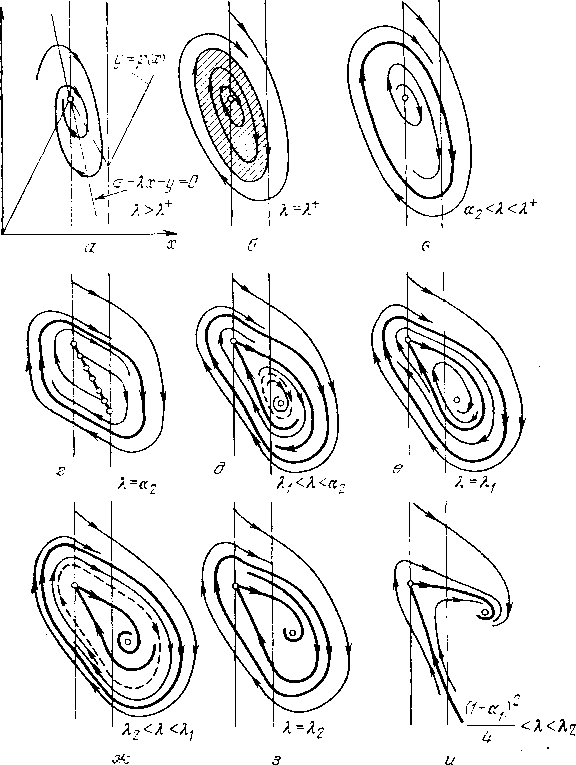
\includegraphics[width=0.6\linewidth]{../img/img215.png}

\setcounter{figure}{1}
\renewcommand{\thefigure}{215}

\caption{}

\label{ris:image}

\end{figure}
Возникает неустойчивый отрезок покоя внутри устойчивого предельного
цикла, При дальнейшем уменьшении $\lambda$ вдоль дискриминантной
кривой появляются два состояния равновесия: склеенный вырожденный 
седло-узел (см. гл. 4, \S 2) и устойчивый фокус в области
\RomanNumeralCaps{3}. От конца отрезка покоя вместе с фокусом рождается неустойчивый 
предельный цикл ($\alpha$-сепаратриса вырождепного состояния 
равновесия идет к устойчивому циклу, охватывающему
все состояния равновесия, $\omega$-сепаратриса скручивается с неустойчивого 
цикла, охватывающего устойчивый фокус (рис. 215, \textit{д})).
Так как $\alpha$-сепаратриса при $\lambda = 0$ (прямая $y = \sigma$) идет в устойчивый 
узел в области \RomanNumeralCaps{3}, состояние равповесия в области \RomanNumeralCaps{3} при
изменении параметров вдоль дискриминантной кривой устойчивости 
не меняет и бесконечность остается неустойчивой, то исчезновение 
предельных циклов на интервале $0 < \lambda < \alpha_{2}$ может
произойти только за счет слияния предельных циклов с последующим 
уничтожением двойного цикла. Это может осуществиться 
лишь при посредстве промежуточной бифуркации — появлении
при $\lambda = \lambda_{1} < \alpha_{2}$ (рис. 215, \textit{е}) потли сепаратрисы, возникшей из
$\alpha$- и $\omega$-сепаратрис сшитого вырожденного состояния равновесия.

Петля сепаратрисы как снаружи, так и изнутри неустойчива.
Такую петлю можно рассматривать как особый предельный цикл
с состоянием равновесия на нем, отделяющий структуры с неустойчивым 
предельпым циклом, охватывающим состояние равновесия 
в области \RomanNumeralCaps{3}, от структур с неустойчивым циклом, охватывающим 
все состояния равновесия.

При убывании $\lambda$ до значения $\lambda = \lambda_{1}$ в петлю «влипает» изнутри 
неусточнвый предельный цикл (рис. 215, \textit{е}), а при дальней
шем убывапии $\lambda$ и разрушении петли от нее рождается неустойчивый 
предельный цикл (рис. 215, \textit{ж}), охватывающий все состояния 
равновесия (а-сепаратриса идет в устойчивый фокус в области 
\RomanNumeralCaps{3}, $\omega$-сепаратриса скручивается с неустойчивого предельного
цикла, который охватывает оба состояния равнонесия, и между
циклами нет состояний равновесия). При некотором $\lambda = \lambda_{2} < \lambda_{1}$,
(рис. 215, \textit{з}) необходимо возникает полуустойчивый двойной предельный 
цикл, исчезающий при убывании $\lambda$. При дальнейшем
убывании $\lambda$ фокусы превратятся в узлы и возпикнет структура,
качественно эквивалентная структуре при $\lambda = 0$ (рис. 215, \textit{и}).
(При убывании $\lambda$ до значения $(1 - \alpha_{1})^2 / 4$ сохрапяется фокус, при
дальнейшем убывании $\lambda$ фокус превращается в узел.)
\end{document}